% Chapter 4

%%%
%\newcommand{\tabhead}[1]{\textbf{#1}}
%%%

\chapter{Elastic deformation} % Main chapter title

\label{Chapter4} % For referencing the chapter elsewhere, use \ref{Chapter1} 
%The elastic deformation is one of the serious systematic error in Photon calibrator.
Calibration of interferometer above 1kHz is a challenging task. 
It was demonstrated that the calibration forces applied by a centered 
photon calibrator beam produce local elastic deformations which 
significantly alter the sensed displacement of the 
interferometer~\cite{Hild:2007,Goetz:2009}.
Even stiff materials like fused silica or sapphire experience small 
deformation when photon calibrator forces are applied. The response to 
the excitation forces can be represented by the appropriate linear 
combination of normal modes. These effects, however, can be mitigated 
by applying at least two beams diametrically opposed and sufficiently 
displaced from the center of the test mass. 
This scheme was tested and implemented in LIGO and advanced LIGO photon 
calibrator~\cite{Daveloza,Karki}.
In this chapter, the investigations to identify 
the modes and their effect on the calibrator performance are discussed.  

The modal analysis and simulation of the elastic deformation are made 
by using Finite Element Analysis (FEA) software package, ANSYS~\cite{ANSYS}. 

%\section{Free mass motion}
%\section{Transfer function}
%\section{Modal analysis}

\section{Perfect Cylinder model}

As the first step, we made the analysis in the perfect cylinder cases.
Table.~\ref{tab:fem_cylpar} shows two sets of parameters similar to LIGO 
and KAGRA end test mass (ETM). 
It is known that two normal modes are most relevant in the calibration 
frequency ranges. The mode resonant frequencies are also shown 
in Table.~\ref{tab:fem_cylpar}.
In the following analysis a cartesian coordniate system is defined 
such that $x-y$ plane is on the circular surface of the cylinder 
and $z$ axis is along the cylinder height.

\begin{table}
\caption{Simulation parameters and resuls for perfect cylinder studies.}
\label{tab:fem_cylpar}
\centering
\begin{tabular}{ccc}
\toprule
\tabhead{Quantity} & \tabhead{LIGO}& \tabhead{KAGRA} \\
\midrule
Diameter [mm] & 340 & 220 \\
Thickness [mm] & 200 & 150.2 \\
Material & Silica & Sapphire \\
Density [kg m$^{-3}$] & 2203 & 4000 \\
Weight [kg] & 40.003 & 22.838 \\
Poisson ratio & 0.1631 & 0.3 \\
Young's modulus [GPa] & 72.6 & 400 \\
Drumhead [Hz] & 8109 & 23798 \\
Butterfly [Hz] & 5969 & 16058 \\
Drumhead node [mm] & 109.0 & 65.3 \\
\bottomrule\\
\end{tabular}
\end{table}

\subsection{Modal displacement parameterization} \label{fem-dpar}

The directional displacements in $z$ component, $\Delta z$ 
can be well approximated by a simple polynomial function.
For the drumhead mode, the displacement, $\Delta z_{DH}$ can be written as:
\begin{equation}
\label{eq:fem-drum}
\Delta z_{DH} = p_0+p_1 r^2+p_2 r^4,
\end{equation}
where $r=\sqrt{x^2+y^2}$ and, $p_0$, $p_1$, $p_2$ are polynomial coefficients.
Figure~\ref{fig:fem-dnode} shows the fitting of FEA results by 
eq.~\ref{eq:fem-drum}. From this fitting we can estimate the 
drumhead node position, $r_{DH}$ as the position where the $z$ displacement 
is equalt to 0.

\begin{figure}
\begin{center}
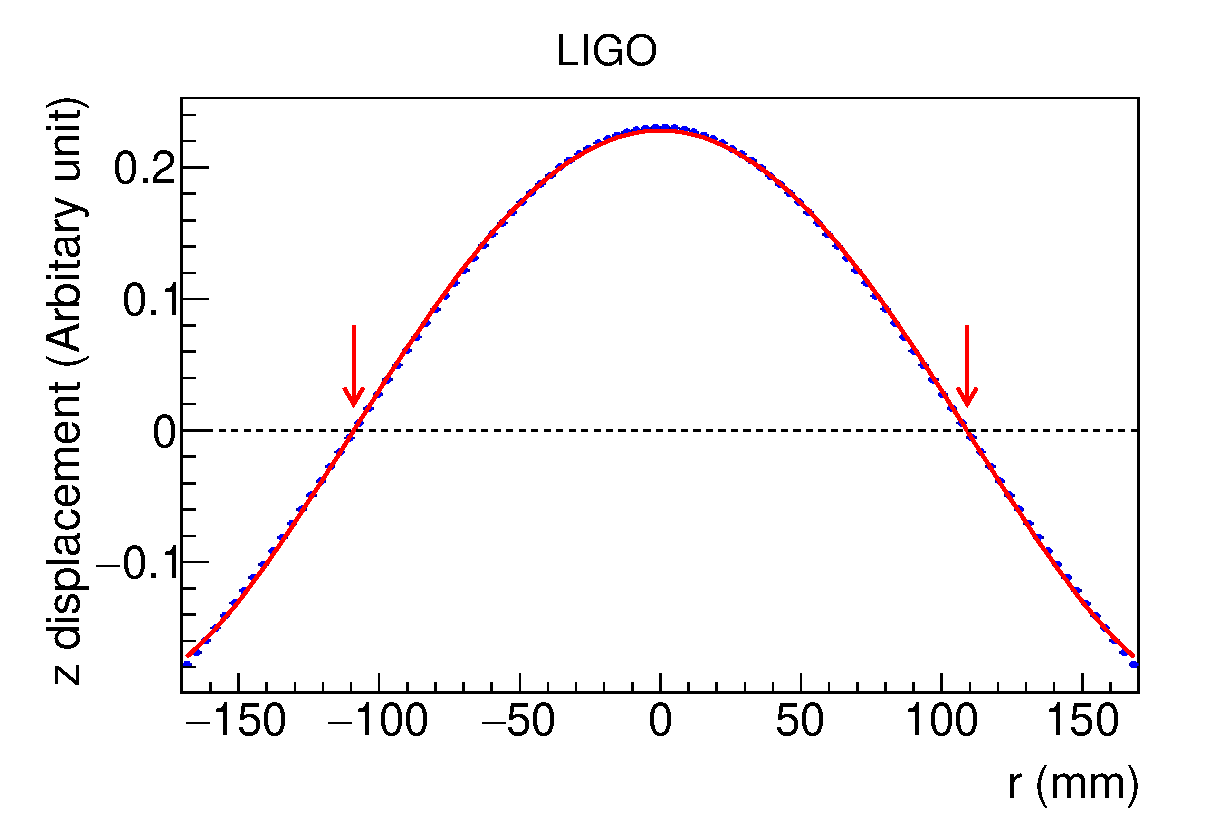
\includegraphics[width=7cm]{Figures/fem-nfit1.eps}
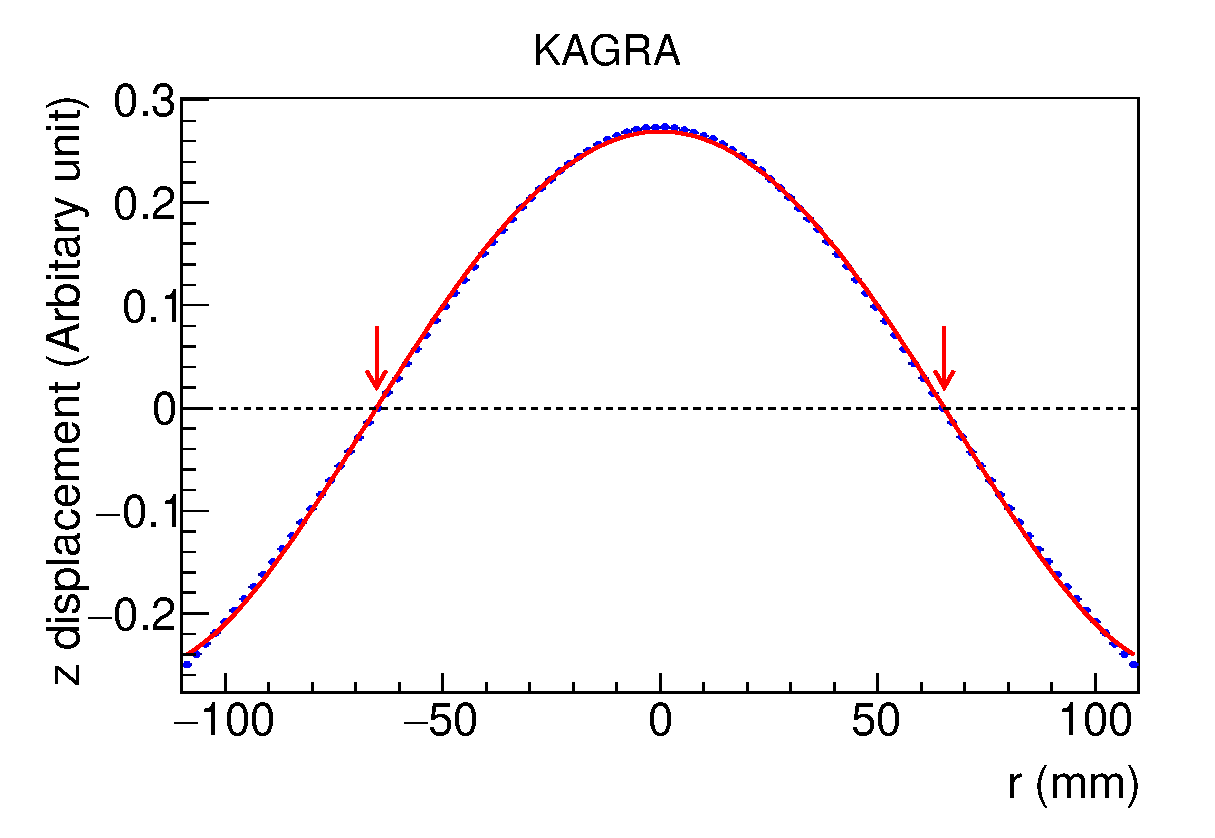
\includegraphics[width=7cm]{Figures/fem-nfit2.eps}
\caption{Fitting of $z$ displacements, $\Delta z_{DH}$ of the drumhead mode 
as a function of $r=\sqrt{x^2+y^2}$ for 
LIGO case (left) and KAGRA case (right). 
The fitted node positions, $r_{DH}$, where $\Delta z_{DH}=0$ 
are 109.0~mm and 65.3~mm for LIGO and KAGRA cases, respectively.} 
\label{fig:fem-dnode}
\end{center}
\end{figure}

For the butterfly mode, the displacement, $\Delta z_{BF}$ 
can be parameterized as:
\begin{equation}
\label{eq:fem-butt}
\Delta z_{BF} = (p_1 r^2+p_2 r^4)\cos(2\theta+\theta_0),
\end{equation}
where $\theta=\arctan(y/x)$ and $\theta_0$ is a phase offset.
Usually, we take $\theta_0=0$ and $\theta_0=\pi/4$ for 
the two butterfly modes. The node lines where $\Delta z_{BF}=0$ lie 
at $\theta=\$theta_0\pm\pi/2$. Fig.~\ref{fig:fem-bfly} shows 
$\Delta z_{BF}=0$ as a function of $r$ and $\theta$ in the LIGO case.
The KAGRA case show very similar behavior.
The four node lines lie at $\theta=\pm1/4\pi$ and $\pm3/4\pi$.

\begin{figure}
\begin{center}
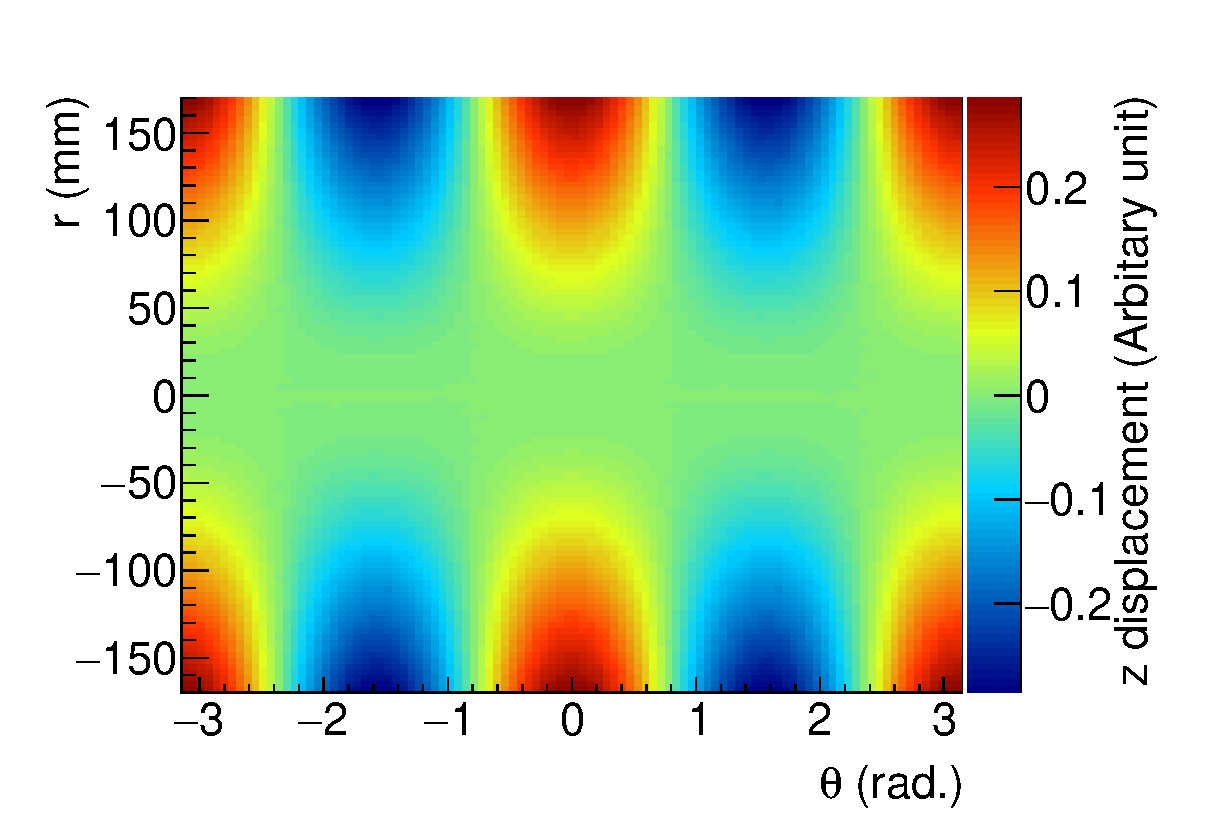
\includegraphics[width=10cm]{Figures/fem-bfly.eps}
\caption{The $z$ displacement, $\Delta z_{BF}$, for the butterfly mode 
as a function of $r=\sqrt{x^2+y^2}$ and $\theta=\arctan(y/x)$
for the LIGO case. The KAGRA case show very similar behavior.
The four node lines lie at $\theta=\pm1/4\pi$ and $\pm3/4\pi$.}
\label{fig:fem-bfly}
\end{center}
\end{figure}

\subsection{Optimal beam position scan} \label{fem-opt}

The total displacement sensed by the main interferometer beam can be 
defined as the combination of the free-mass motion and the surface 
displacement due to the elastic deformation. The free-mass motion, 
$D_{\rm free}$ 
can be written as
\begin{equation}
D_{\rm free}(f) = \frac{F}{m(2\pi f)^2},
\end{equation}
where $F$ is an external force, $m$ is the mirror mass and 
$f$ is the frequency.

In the coordinate system that $z$-axis is along the main interferometer 
beam, the effective displacement sensed by the main interferometer beam,
$D_{\rm eff}(f)$ is represented by the surface integral on the HR plane, 
of the test mass, $\Omega_{\rm HR}$ :
\begin{equation}
D_{\rm eff}(f) = k_{I}\int_{\Omega_{\rm HR}}D(x,y;f)I(x,y){\rm d}x{\rm d}y,
\end{equation}
where $D(x,y;f)$ is the total displacement at $(x,y)$ for frequency $f$, 
$I(x,y)$ is the interferometer beam profile, 
\begin{equation}
I(x,y) = \exp\left(-2\frac{x^2+y^2}{r_{\rm beam}^2}\right),
\end{equation}
and $k_{I}$ is a normalization constant defined as:
\begin{equation}
k_{I}\int_{\Omega_{\rm HR}}I(x,y){\rm d}x{\rm d}y = 1.
\end{equation}

In case of LIGO, $r_{\rm beam}=$ 62~mm and $k_{I}=$ 165.614~m$^{-2}$.
In case of KAGRA, $r_{\rm beam}=$ 35.3~mm and $k_{I}=$ 2893.36~m$^{-2}$.
Finally, the displacement ratio, $R(f)$ is defined as:
\begin{equation}
R(f) = \frac{D_{\rm eff}(f)}{D_{\rm free}(f)}.
\end{equation}

Fig.~\ref{fig:fem-optc} shows the displacement ratio, $R(f)$ 
as a function fo frequency, $f$ for optimally positioned beams and 
$\pm$2 mm and $\pm$4 mm offsets for LIGO case and KAGRA case. 
The cross check of the simulation is also done with COMSOL~\cite{COMSOL} 
and the agreement within 0.2~\% has been obtained.

\begin{figure}
\begin{center}
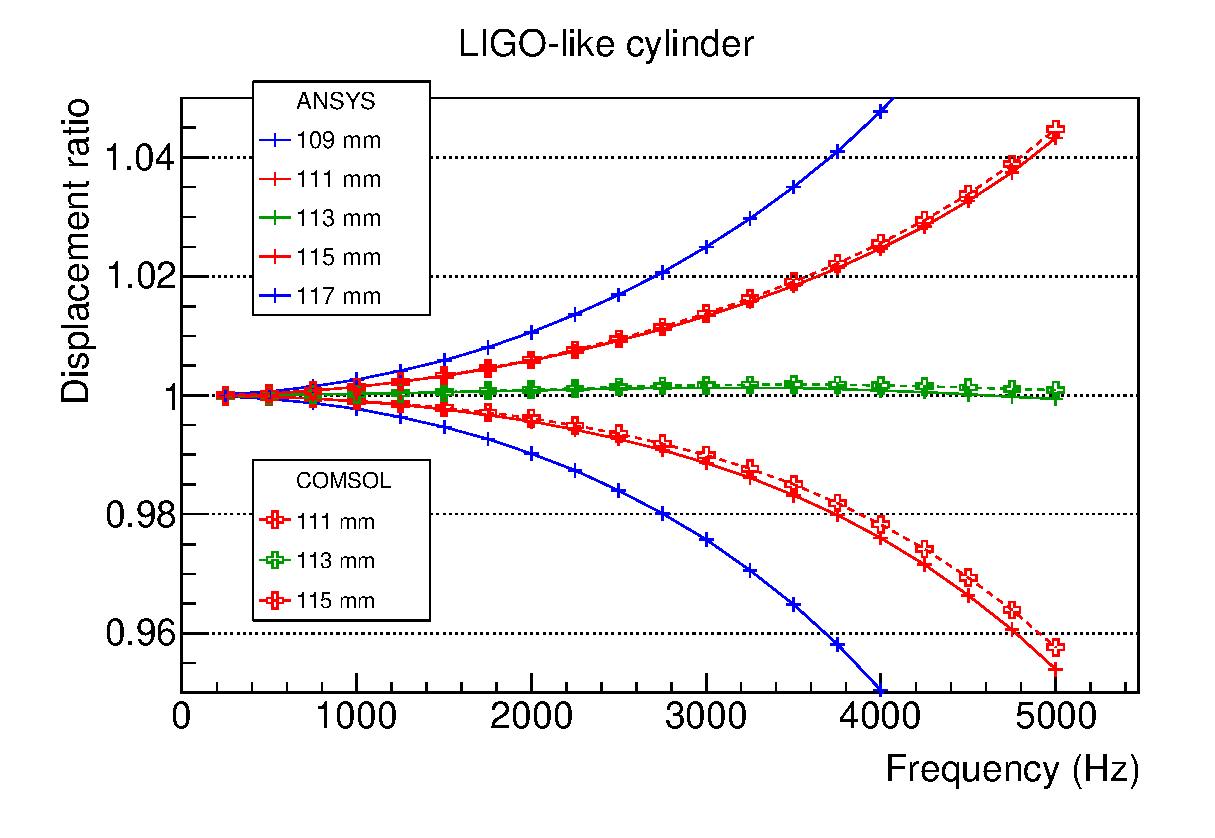
\includegraphics[width=12cm]{Figures/fem-lgc-opt.eps}
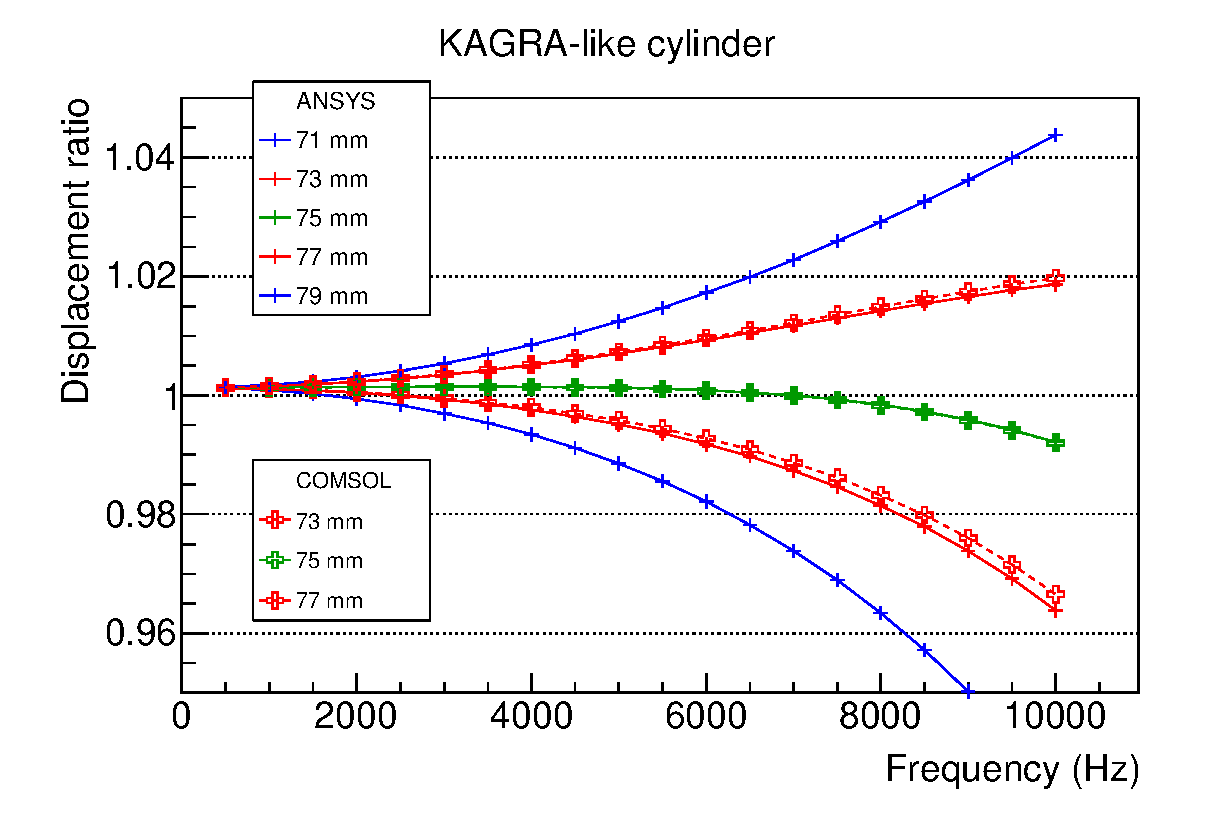
\includegraphics[width=12cm]{Figures/fem-kgc-opt.eps}
\caption{The ratio, $R(f)$ between the total sensed motion, 
$D_{\rm eff(f)}$ and free mass motion, $D_{\rm free}(f)$ 
as a function of frequency, $f$ for optimally positoned beams and 
$\pm$2 mm and $\pm$4 mm offsets for (top) LIGO case and 
(bottom) KAGRA case. The cross check of the simulation is also done 
with COMSOL~\cite{COMSOL} and shown for optimum positoin and $\pm$2 mm 
offsets with open cross symbols.} 
\label{fig:fem-optc} 
\end{center}
\end{figure}


\section{Real ETM model}

The real structure of KAGRA ETM is not a perfect cylinder but 
has two flat cuts at both sides with two ears used to hang the mirror. 
Fig.~\ref{fig:fem-etm} 
shows the CAD model of the KAGRA ETM. We made the similar FEA on the 
realistic KAGRA ETM structure. The results are shown in 
Table.~\ref{tab:fem-etm}, which are very close to those 
obtained in the perfect cylinder model.
Fig.~\label{fig:fem-etm-mode} shows the illustration of 
$z$ displacements for two dominant modes, butterfly and drumhead modes.
One particular effect in KAGRA ETM is that it is not symmetric in
vertical direction along $y$-axis. Fig.~\ref{fig:fem-dnetm}

\begin{figure}
\begin{center}
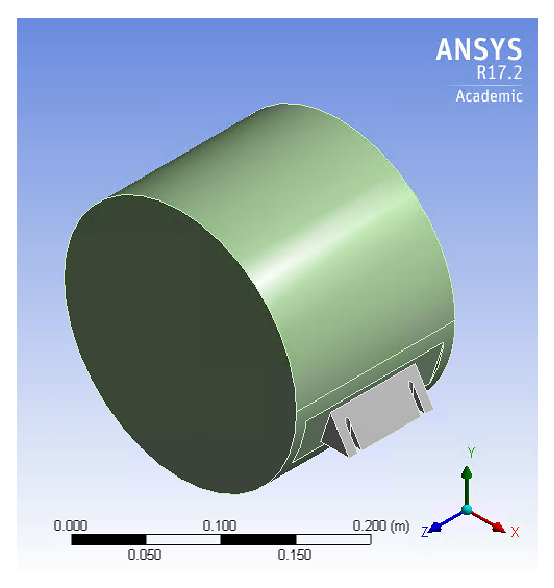
\includegraphics[width=10cm]{Figures/fem-etm.eps}
\caption{The CAD model of the KAGRA ETM with flat cuts and ears.}
\label{fig:fem-etm}
\end{center}
\end{figure}

%Figure~\ref{fig:elmodes} shows the summary of primary modes, drumhead and 
%butterfly modes compared between KAGRA and LIGO.
We made the same analysis as in Section~\ref{fem-opt} to obtain 
the optimal position of beams. 
Figure~\ref{fig:fem-opte} shows the displacement between the sensed motion 
and free mass motion as a function of frequency for optimally positioned 
beams on KAGRA test mass, as well as $\pm$1 mm and $\pm$3 mm offsets from 
the optimal positions.

\begin{table}
\caption{Simulation parameters and resuls for the KAGRA ETM CAD model.}
\label{tab:fem-etm}
\centering
\begin{tabular}{ccc}
\toprule
\tabhead{Quantity} & \tabhead{Cylinder} & \tabhead{CAD model} \\
\midrule
Diameter [mm] & 220 & 220 \\
Thickness [mm] & 150.2 & 150.2 \\
Material & Sapphire & Sapphire \\
Density [kg m$^{-3}$] & 4000 & 4000 \\
Weight [kg] & 22.838 & 22.994 \\
Poisson ratio & 0.3 & 0.3 \\
Young's modulus [GPa] & 400 & 400 \\
Drumhead [Hz] & 23798 & 23658 \\
Butterfly [Hz] & 16058 & 15913 \\
Drumhead node [mm] & $\pm$65.3 & -66.5/62.7 \\
\bottomrule\\
\end{tabular}
\end{table}

\begin{figure}
\begin{center}
\includegraphics[width=12cm]{Figures/kg-etm-dh.eps}
\includegraphics[width=12cm]{Figures/kg-etm-bf.eps}
\caption{Drumhead (top) and Butterfly (bottom) modes for KAGRA ETM.}
\label{fig:fem-etm-mode}
\end{center}
\end{figure}

\begin{figure}
\begin{center}
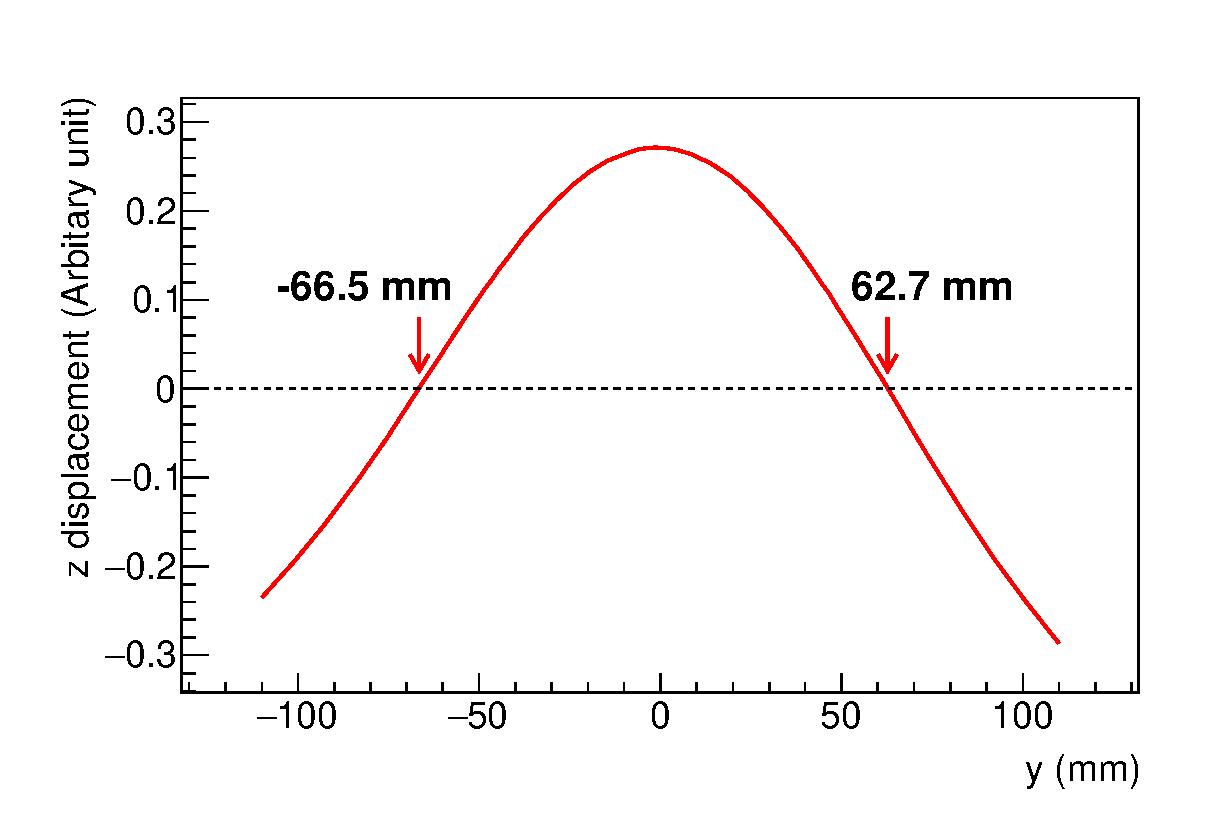
\includegraphics[width=12cm]{Figures/fem-nfit3.eps}
\caption{Fitting of $z$ displacements, $\Delta z_{DH}$ of the drumhead mode 
as a function of $y$ for KAGRA ETM model.
The fitted dnode positions, $r_{DH}$, where $\Delta z_{DH}=0$ 
are asymmetric and located at -66.5~mm and 62.7~mm.} 
\label{fig:fem-dnetm}
\end{center}
\end{figure}

%\begin{figure}
%\begin{center}
%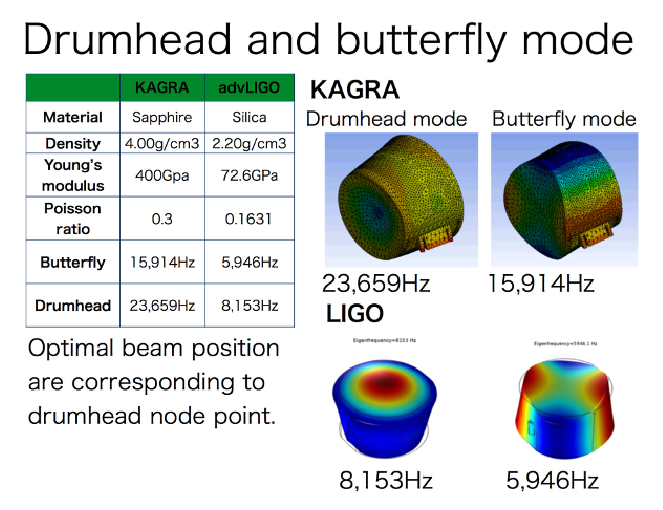
\includegraphics[width=14cm]{Figures/elmodes.eps}
%\caption{Summary of drumhead and butterfly modes on KAGRA test mass 
%compared with LIGO test mass.~\cite{Daveloza}} 
%\label{fig:elmodes} 
%\end{center}
%\end{figure}

\begin{figure}
\begin{center}
%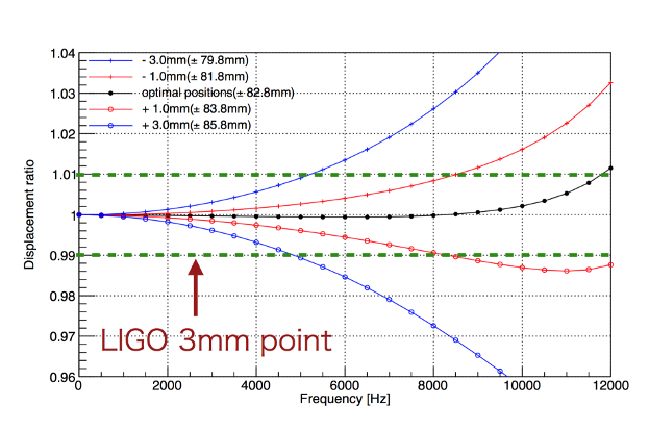
\includegraphics[width=14cm]{Figures/edeform.eps}
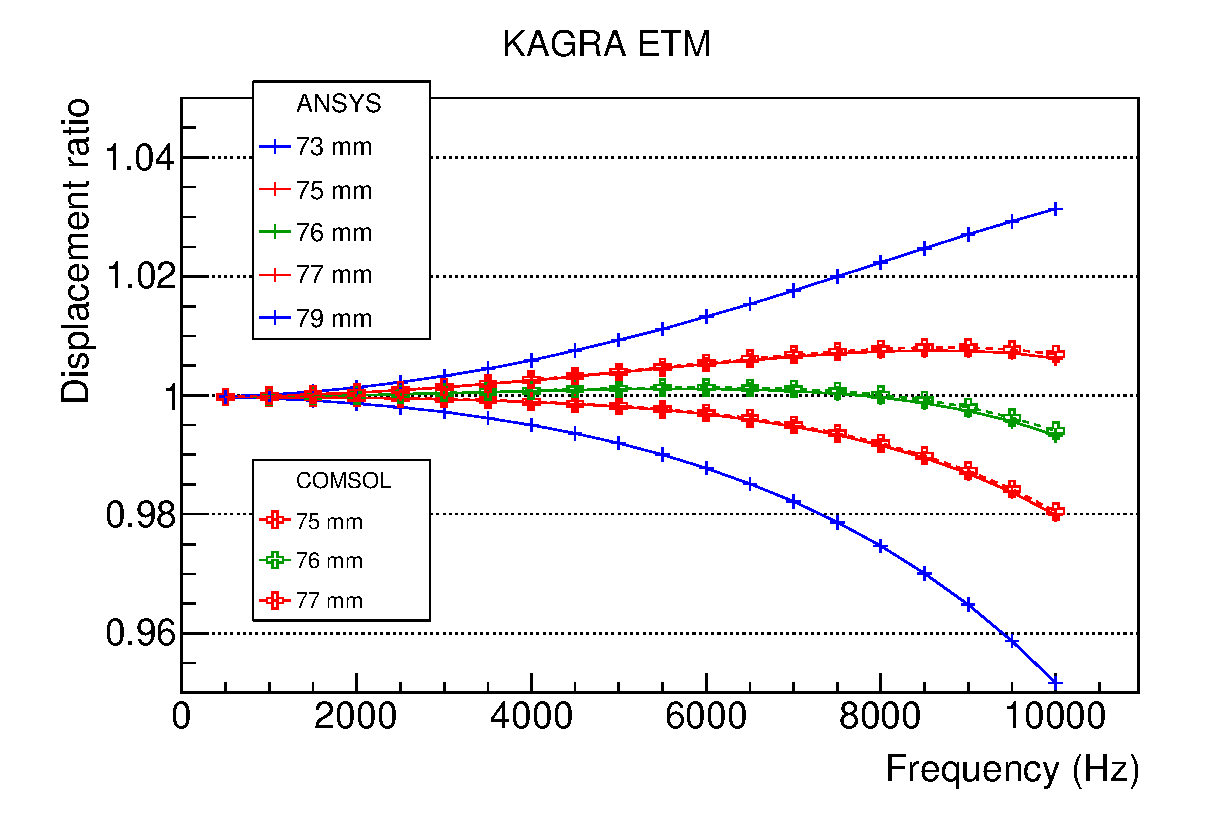
\includegraphics[width=12cm]{Figures/fem-kge-opt.eps}
\caption{The ratio between the total sensed motion and rigid body motion 
as a function of frequency for optimally positioned baams and 
$\pm$1 mm and $\pm$3 mm offsets. The cross check of the simulation 
is also done with COMSOL~\cite{COMSOL} and shown for optimum position 
and $\pm$1 mm offsets with open cross symbols.} 
\label{fig:fem-opte} 
\end{center}
\end{figure}

%\section{Elastic deformation}
%\section{Summary}
